\documentclass[12pt,a4paper,twoside,openright]{book}
\usepackage[T1]{fontenc}
\usepackage[utf8]{inputenc}
\usepackage[italian]{babel}
\usepackage[colorlinks=false, linktocpage=true]{hyperref}
\usepackage{makeidx}
\usepackage[nottoc,notlot,notlof]{tocbibind}
\usepackage[autostyle,italian=guillemets]{csquotes}
\usepackage[backend=biber,sorting=none]{biblatex}
 \addbibresource{bibliografia-tesi.bib}
\usepackage{amsmath}
\usepackage{amsfonts}
\usepackage{amssymb}
\usepackage{frontespizio}
\usepackage{fancyhdr}
\usepackage{indentfirst}
\usepackage{bold-extra}
\usepackage{bookmark}
\usepackage{lmodern}
\usepackage{etoolbox}
\usepackage{wrapfig}
\usepackage{color}
\usepackage{graphicx}
\usepackage{fancyref}
\usepackage[titletoc,title]{appendix}

\usepackage{nameref}

\usepackage[section]{placeins}

\patchcmd{\chapter}{\thispagestyle{plain}}{\thispagestyle{fancy}}{}{}

\makeindex

\newenvironment{abstract}% 
	{\cleardoublepage%
		\thispagestyle{empty}%
		 \null \vfill\begin{center}%
			\bfseries \abstractname \end{center}}% 
	{\vfill\null}

\newcommand{\nrange}[4][]{%
  #2=%
  \ifblank{#1}{% Optional argument empty? Yes? Then omit the second number in the enumeration
    #3, \dots ,#4%
  }{%
    #3, #1, \dots,#4%
  }%
}

\newcommand{\fncyfront}{% 
	\fancyhead[RO]{{\footnotesize\rightmark}} 
	\fancyfoot[RO]{\thepage} \fancyhead[LE]{\footnotesize{\leftmark}} 
	\fancyfoot[LE]{\thepage} 
	\fancyhead[RE,LO]{}
	\fancyfoot[C]{}
	\setlength{\headheight}{14.5pt}
\renewcommand{\headrulewidth}{0.3pt}}

\newcommand{\fncymain}{%
	\fancyhead[RO]{{\bfseries\footnotesize\rightmark}} 
	\fancyfoot[RO]{\bfseries\thepage} 
	\fancyhead[LE]{{\bfseries\footnotesize\leftmark}} 
	\fancyfoot[LE]{\bfseries\thepage}
	\fancyfoot[C]{} 
	\setlength{\headheight}{26pt}
\renewcommand{\headrulewidth}{2pt}}


\makeatletter
\def\cleardoublepage{\clearpage\if@twoside \ifodd\c@page \else\hbox{}\thispagestyle{empty}\newpage
\if@twocolumn\hbox{}\newpage\fi\fi\fi} \makeatother

\author{Daniel Casenove}
\title{Rilevazione di disservizi nella connettività di rete}



\begin{document}
\pagestyle{fancy}
\fncyfront
\frontmatter
\begin{frontespizio}
\Margini{2.5cm}{1.5cm}{2.5cm}{1cm}
\Istituzione{Università di Pisa}
%\Facolta{SCIENZE MATEMATICHE, FISICHE E NATURALI}
\Dipartimento{Informatica}
\Corso[Laurea Triennale]{Informatica}
\Titoletto{Tesi di Laurea Triennale}
\Titolo{Rilevazione di disservizi nella connettività di rete}
\Logo[2.5cm]{images/cherubino_pant541}
\Candidato{Daniel Casenove} \Relatore{Luca Deri} 
\Annoaccademico{2018/2019}
\end{frontespizio}

\begin{abstract}
 
\end{abstract}
\pagenumbering{gobble}

\tableofcontents
%\thispagestyle{empty}
\fncymain
\mainmatter
\pagenumbering{arabic}

%\flushbottom
\raggedbottom
\chapter{Introduzione}

Nell'ultimo decennio, con la crescita in popolarit\`a degli smartphone, si \'e assistito ad un aumento e ad una diversificazione di dispositivi connessi in rete senza precedenti.
Una tipica rete non \'e pi\`u composta semplicemente da qualche PC e server, in caso aziendale, ma anche da telefoni, tablet, smart TV, weareables ed elettrodomestici.
Inoltre non \'e poi cos\`i raro per un utente possedere pi\`u di uno di questi device, aumentando drasticamente il numero di apparecchiature collegate in una singola rete.
Secondo previsioni Cisco, il numero di dispositivi connessi a reti IP sar\`a pari al triplo del numero della popolazione globale entro il 2022\cite{CVI}.
Lo stesso studio riporta un forte cambiamento nel tipo di dispositivi connessi, con dispositivi mobili quali smartphone e tablet, sistemi embedded in TV ed elettrodomestici in costante crescita a discapito dei pi\`u tradizionali PC.
Viene stimato che, entro il prossimo triennio, il 51\% dei dispositivi e connessioni saranno di tipo machine-to-machine, ovvero senza interazione umana, e principalmente costituiti da device IoT\cite{CVI}.
Data la natura dei dispositivi in crescita nelle reti, si osserva anche un cambiamento nel mezzo trasmissivo in favore della connessione senza fili a discapito della connessione cablata\cite{CVI}.

In contemporanea all'aumento del numero di dispositivi connessi ad Internet si \'e assistito anche ad un cambio nel paradigma di erogazione di servizi in favore del cloud computing e cloud storage.
Ad esempio, servizi come Google Drive e Dropbox permettono di salvare i propri file in remoto ed accederne tramite connessione ad Internet, diminuendo l'uso di memoria nel dispositivo personale a discapito della necessit\`a di connessione performante.
Allo stesso modo, servizi di streaming come Netflix e Spotify forniscono cataloghi multimediali pressoch\`e infiniti.

In un mondo sempre pi\`u connesso digitalmente diventa quindi fondamentale, per una rete locale, essere in grado di sostenere un traffico di dati elevato ed un numero di dispositivi in costante crescita in modo da poter fornire una buona connettivit\`a per una corretta esperienza d'uso.

Sebbene gran parte del traffico verso questi tipi di servizi venga generato tramite connessioni mobili, quali 3G e 4G, queste non saranno oggetto di discussione.
Il motivo principale risiede nel fatto che la qualit\`a della connessione, in questo caso, dipende quasi interamente dalla bont\`a del segnale ricevuto dalle antenne dell'operatore.
Incidono anche fattori metereologici \cite{inproceedings}, il posizionamento delle apparecchiature sul territorio e la loro rispettiva capillarit\`a.
Fattori secondari di qualit\`a del segnale possono essere invece ricondotti alle antenne del dispositivo mobile che usufruisce della connessione ma, anche in questo caso, esse vengono scelte dal fabbricante e quindi sono fuori dal controllo dell'utente.
I temi affrontati da questo elaborato riguardano la qualit\`a del servizio offerto da reti locali e dei dispositivi collegati ad esse.
Gli sviluppi nel mondo tecnologico precedentemente citati hanno dato vita a diverse sfide per fabbricanti di apparecchiature di rete e personale specializzato del settore.
Ad esempio, l'introduzione della connessione senza fili, richiede particolare attenzione per via della natura delle onde radio.
Gli access point devono essere posizionati in modo strategico all'interno del locale dove si vuole instaurare la connessione, tenendo conto di problemi come l'attenuazione del segnale attraverso mura \cite{6971137} e interferenze causate con altri dispositivi attivi sulla stesse frequenze.
%Posizionamento tramite algoritmi
Una soluzione al primo problema si trova nel posizionare apparecchiature come repeater per estendere il campo di copertura mentre l'utilizzo di software professionale pu\`o essere necessario per la scelta corretta di un canale libero da interferenze.
L'aumento vertiginoso del numero dei dispositivi connessi alle reti aumenta anche l'importanza di riuscire di riuscire a capirne il tipo ed eventuali servizi offerti prima di iniziare una fase di monitoraggio riguardante il traffico di rete.
Ci sono diverse tecniche in letteratura per questo tipo di analisi, sia di tipo attivo che passivo, che verranno presentate ed approfondite nel prossimo capitolo.
Questo tipo di studio, come vedremo, \'e fondamentale per fornire una corretta analisi dei disservizi di una rete locale poich\`e \'e necessario, prima di tutto, avere un'idea della quantit\`a e del tipo dei dispositivi che si andranno a monitorare.
In un secondo momento verranno poi presentati alcuni strumenti per il monitoraggio effettivo della rete che, anche in questo caso, possono essere divisi in passivo o attivo.
Purtroppo le principali limitazioni di questo tipo di strumenti includono l'implementazione in sole apparecchiature professionali e la difficolt\`a d'uso per personale non specializzato.
Lo studio si \'e quindi incentrato sulla possibilit\`a di implementare tecniche per la rilevazione di disservizi in reti locali tenendo in mente la facilit\`a d'uso e la possibilit\`a di implementazione su apparecchiature a basso costo per reti di piccole dimensioni.
%Si vuole inoltre fornire all'utente una localizzazione del problema in rete e cos

%Modem router moderni

%Topologia
%Utile in ambito aziendale?

%Queste soluzioni, per ora brevemente accennate, sono per\`o principalmente rivolte ad un ambito aziendale dato il costo delle apparecchiature che le implementano e la necessit\`a di personale specializzato in grado di farne uso.


%Cambiamento alle reti locali grazie al wifi
%Posizionamento router,repeater
%Cavo
%Differenze con reti casalinghe
%Device che vanno e vengono

%I temi che verranno affrontati riguardano la qualit\`a del servizio di reti locali e dei dispositivi collegati ad esse.

%Questo fenomeno introduce un'altra serie di problemi legati alla natura delle onde radio come attenuazione del segnale dovuto alle mura di edifici ed interferenze con altri dispositivi che offrono connessione Wi-Fi.

%Fruibilita' tramite internet 
%Non si parla di reti mobili
%PROBLEMA
%SOLUZIONE
%PER CHI NON VA LA SOLUZIONE

%Per garantire un operato corretto della rete, le apparecchiature di rete di fascia alta sono dotate di funzioni di monitoraggio che aiutano l'utente nella rilevazione di disservizi.
%Data la natura tecnica del problema ed il costo di tali apparecchiature l'uso di queste soluzioni \'e per\`o principalmente ristretto a reti aziendali e di grandi dimensioni, dove personale specializzato ha il compito di instaurare e supervisionare la rete.


\section{Obiettivo}

Lo scopo di questo elaborato \'e quello di fornire uno strumento in grado di rilevare eventuali disservizi nella connettivit\`a di piccole reti locali dove le apparecchiature presenti non sono dotate di funzioni di monitoraggio.
La crescita non omogenea di questo tipo di reti, il numero spesso imprevedibile di dispositivi connessi e la moltitudine di servizi che questi offrono, rendono, per\`o, necessaria anche una prima analisi di rete finalizzata a determinare la quantit\`a ed il tipo di device connessi.
Successivamente, con metriche che verranno introdotte nei prossimi capitoli, si procede al monitoraggio di tutti i dispositivi appartenenti alla rete. 
In particolare, in caso di malfunzionamenti, si vuole identificare se questi siano dovuti a problematiche interne alla propria Local Area Network (LAN) o alla Wide Area Network (WAN) del provider Internet.
Per disservizi interni alla LAN, successivamente alla localizzazione del problema, si procede proponendo soluzioni all'utente e identificando tutti i dispositivi il cui servizio \'e degradato.
%L'aumento vertiginoso del numero dei dispositivi connessi alle reti aumenta anche l'importanza di riuscire di riuscire a capirne il tipo ed eventuali servizi offerti prima di iniziare una fase di monitoraggio riguardante il traffico di rete.


\section{Contributo personale}

Durante lo studio iniziale si \'e notata la mancanza di strumenti open-source in grado di fornire una visione topologica dei dispositivi Wi-Fi.
Si \`e quindi sviluppata una libreria in grado di monitorare, tramite ispezione di frame 802.11, il traffico Wi-Fi delle reti circostanti per poi fornirne dati relativi alla potenza del segnale dei dispositivi connessi ed una topologia dettagliata.
Questo passaggio permette il discovery di dispositivi Wi-Fi nella nostra rete locale ed un monitoraggio nel tempo della bont\`a del segnale.
I dettagli implementativi e la relativa validazione sono lasciati ai corrispettivi capitoli dell'elaborato.

\newpage

\section{Struttura della tesi}

La tesi \'e divisa in cinque capitoli di cui si elenca un breve sommario:

\begin{itemize}
	\item Capitolo 1: \textbf{Introduzione}, vengono presentati il problema analizzato e le motivazioni che hanno portato alla stesura di questa tesi.
	\item Capitolo 2: \textbf{Stato dell'arte}, vengono descritte le attuali tecnologie utilizzate per la rilevazione di disservizi nella connettivit\`a di rete.
	\item Capitolo 3: \textbf{Soluzione proposta}, vengono esposte la soluzione proposta e la libreria sviluppata. 
	\item Capitolo 4: \textbf{Validazione}, vengono mostrati i risultati ottenuti al fine di validare la soluzione proposta.
	\item Capitolo 5: \textbf{Conclusione e lavoro futuro}, presentazione delle conclusioni raggiunte ed alcune ipotesi per lavori futuri.
\end{itemize}
%\raggedbottom
\chapter{Stato dell'arte}
In questo capitolo vengono presentate le motivazioni che hanno portato alla stesura di questo elaborato e le soluzioni per rilevazione di disservizi nella connettivit\`a pi\'u utilizzate.

\section{Motivazione}
Come introdotto nel precedente capitolo, lo scopo di questo lavoro \'e di fornire una soluzione per la rilevazione di disservizi in reti locali domestiche.
Lo studio si \'e focalizzato su questo tipo di infrastrutture poich\`e esse rappresentano la maggioranza delle reti e, molto spesso, la loro configurazione \'e  lasciata ad un utente finale con poche conoscenze del campo.
Questo pu\`o portare a prestazioni poco efficienti per quanto riguarda le connessioni Wi-Fi o all'uso di apparecchiature di scarsa qualit\`a che dimuiscono le velocit\`a di download ed upload dei dispositivi.
In aggiunta, access point vicini, se sullo stesso canale Wi-Fi,potrebbero interferire sulla connessione locale.
Per questo motivo, software come Kismet\cite{kismet}, possono essere utilizzati anche per scegliere un canale non sovrautilizzato oltre a monitorare il traffico Wi-Fi ed i device connessi ad una rete.
Negli ultimi tempi, i produttori di router, stanno cercando di implementare in tutti i loro dispositivi metodi di monitoraggio per rilevare disservizi di reti.
Questo permette agli Internet Service Providers (ISP) di fornire una diagnostica iniziale che circoscriva il problema all'interno o all'esterno della rete.
Nel primo caso, l'utente viene informato della presenza del problema nella sua rete locale e quali dispositivi ne siano affetti, mentre nel secondo caso \'e il fornitore del servizio Internet a dover intervenire sulla propria rete per rimediare al disservizio.
Le soluzioni attuali per il monitoraggio e la gestione di rete presentano infatti diverse problematiche quando applicate a reti piccole locali.
\newpage
%In particolare, sono principalmente ristrette ad apparecchiature di fascia alta, molto lontane da quelle fornite dai provider Internet ai loro utenti.
%Le soluzioni attuali per il monitoraggio e gestione di rete, come ad esempio SNMP\cite{rfc1157}, sono infatti principalmente ristrette ad apparecchiature di fascia alta, molto lontane da quelle fornite dai provider Internet ai loro utenti.
%In altri casi, anche alcune funzionalit\`a come il rilevamento di rete CDP sono proprietarie o funzionanti solo con apparati dello stesso produttore.
In particolare il software \'e:
\begin{itemize}
	\item Ristretto ad apparecchiature di fascia alta.
	\item Non sempre fornito di interoperabilit\`a con software di altri produttori.
	\item Difficile da utilizzare per personale non specializzato.
\end{itemize}

Per questi motivi l'elaborato vuol fornire, dopo aver introdotto le tecniche di rilevazione di disservizi pi\`u comuni, una soluzione che possa essere utilizzata in piccole reti da utenti non esperti e su apparecchiature non professionali.

\section[IEEE 802.11 Distributed Coordination Function]{IEEE 802.11 \\Distributed Coordination Function}
Nel protocollo 802.11 il meccanismo di accesso al mezzo trasmissivo \'e chiamato distributed coordination function (DCF) \cite{ieee99}.
Questo metodo di accesso casuale \'e basato sul protocollo di accesso multiplo tramite rilevamento della portante con evitamento delle collisioni (CSMA/CA) in cui i terminali tentano di evitare a priori il verificarsi di collisioni durante la trasmissione.
La ritrasmissione, in caso di collisione di pacchetti, \'e gestita tramite un algoritmo di backoff esponenziale binario (BEB) che verr\`a presentato in dettaglio successivamente.
\'E importante notare che lo standard IEEE 802.11 definisce anche un  protocollo opzionale ,chiamato point coordination function (PCF), in cui l'access point ha il compito di coordinare l'accesso al mezzo trasmissivo per evitare collisioni. 
Questo tipo di meccanismo di accesso non verr\`a trattato per via del suo poco utilizzo.

DCF descrive due tecniche per la trasmissione di pacchetti:
\begin{itemize}
 \item Two-way handshake: meccanismo di accesso base.
 \item Four-way handshake: request to send/clear to send (RTS/CTS).
\end{itemize}

Il meccanismo di accesso base \'e ottenuto attraverso la trasmissione immediata di un acknowledgment positivo (ACK) da parte della stazione destinataria dopo aver ricevuto correttamente un pacchetto dal mittente.
L'invio esplicito dell'ACK \'e richiesto poich\`e in un mezzo trasmissivo senza fili il mittente non pu\`o determinare se il pacchetto sia stato ricevuto correttamente ascoltando la sua stessa trasmissione.

Il meccanismo RTS/CTS \'e opzionale e prevede che una stazione interessata all'invio di un pacchetto riservi il mezzo tramite un pacchetto request to send.
Dopo che il destinatario riconosce questo pacchetto con un frame CTS la comunicazione continua con l'invio del pacchetto desiderato e di relativo ACK.

Questo meccanismo permette l'incremento della performance del sistema grazie alla riduzione della durata di collisione che potrebbe avvenire con l'invio di lunghi pacchetti.
Infatti, in questo caso, la collisione pu\`o solamente avvenire sul frame RTS e viene riconosciuta dalla mancanza di un frame CTS di risposta del destinatario.
In aggiunta il meccanismo RTS/CTS implementato nello standard IEEE 802.11 \'e sviluppato per contrastare il problema dei terminali nascosti \cite{tobagi1975packet} che si presenta quando un paio di stazioni mobili non riescono a rilevarsi. %Migliorare questa parte, aggiungere reference

Si presenta ora il funzionamento di DCF, come standardizzato dal protocollo 802.11.

Una stazione che vuole trasmettere un pacchetto, prima di inviarlo, monitora l'attivit\`a presente sul canale.
Se il canale risulta inattivo per una durata pari ad un distributed interframe space (DIFS), il mittente procede all'invio del frame.
In caso contrario, se il canale \'e attualmente in uso, la stazione continua a monitorarlo finch\`e esso non risulta inattivo per un DIFS.
A questo punto la stazione attende per un intervallo casuale di backoff per minimizzare la probabilit\`a di collisione di pacchetti con altre stazioni che hanno intenzione di trasmettere.
Nello stesso modo, una stazione dovr\`a attendere un altro intervallo casuale per l'invio di due pacchetti consecutivi, anche se il canale risulta inattivo per un DIFS in modo da non impossessarsi del canale di trasmissione.
L'uso del backoff casuale \'e il meccanismo che questo protocollo implementa per la collision avoidance.

DCF utilizza una scala a tempo discreto di backoff per motivi di efficienza, infatti il tempo immediatamente successivo ad un DIFS viene diviso in slot ed ogni stazione pu\`o solo trasmettere all'inizio di ciascuno di questi.
\begin{wraptable}{r}{6cm}
%\begin{flushright}
\centering
\begin{tabular}{| l | l | l | l |}
	\hline 
	PHY & $\delta$ & CW\textsubscript{min} & CW\textsubscript{max} \\ \hline
	FHSS & 50 & 16 & 1024 \\ \hline
	DSSS & 20 & 32 & 1024 \\ \hline
	IR &8 & 64 & 1024 \\ 
	\hline
\end{tabular}
%\end{flushright}
\caption{Tabella 1}
\label{table:deltavalues}
\end{wraptable}

La dimensione dello slot, $\delta$,  \'e pari al tempo che una stazione impiega per rilevare la trasmissione di un pacchetto da parte di una qualsiasi altra stazione.
Questo valore dipende dal tipo dal tipo del mezzo trasmissivo e viene raffigurato nella tabella \ref{table:deltavalues}.
Come precedentemente introdotto, DCF, implementa un backoff esponenziale ed il tempo viene scelto in un range (0, $\omega$-1) dove $\omega$ \'e detta contention window.
Questo valore dipende dal numero di trasmissioni fallite per un pacchetto, a partire da un valore pari a CW\textsubscript{min}  viene raddoppiata ad ogni trasmissione fallita fino ad un valore massimo pari a CW\textsubscript{max}=2\textsuperscript{m} CW\textsubscript{min}.
I valori minimi e massimi della finestra sono specificati, a seconda del tipo di mezzo di trasmissione, nella tabella \ref{table:deltavalues}.
Il contatore del backoff viene decrementato quando il canale si trova in uno stato di idle mentre \'e mantenuto inalterato quando una trasmissione viene captata sul canale.
Infine, la stazione trasmette quando il valore del contatore raggiunge lo 0.

Si presentano ora due esempi di trasmissione usando i due metodi di accesso al metodo trasmissivo presentati.

Considerando due stazioni A e B che condividono lo stesso canale utilizzando il metodo base di accesso, alla fine della trasmissione B attende un DIFS e sceglie un tempo di backoff prima di trasmettere un nuovo pacchetto.
Durante questo periodo la stazione A invia un pacchetto sul canale e, di conseguenza, il timer di backoff della stazione B rimane invariato fino a che il canale non verr\`a percepito come libero per almeno un DIFS.
Per quanto riguarda la stazione A, essa riceve un ACK per segnalare la ricezione con successo del pacchetto da parte del destinatario.
Il pacchetto di ACK viene inviato immediatamente trasmesso alla fine del messaggio, dopo un periodo di attesa chiamato short interframe space (SIFS).
La durata di un SIFS \'e inferiore a quella di un DIFS, questo rende impossibile alle altre stazioni di rilevare come libero il canale fino a che non venga inviato l'ACK.
In caso di mancata ricezione dell'ACK da parte della stazione A entro un tempo specificato ACKTimeout o della trasmissione di altri pacchetti nel canale, questa rischedula l'invio del pacchetto tramite le regole di backoff presentate.

Nel meccanismo RTS/CTS una stazione che vuole trasmettere un pacchetto aspetta fino a che non rileva il canale inattivo per un DIFS, segue le regole di backoff precedentemente introdotte e trasmette un frame speciale chiamato RTS.
Quando la stazione ricevente riconosce un frame RTS risponde, dopo un SIFS di attesa, con un frame CTS.
Il mittente \'e autorizzato ad utilizzare il canale solo alla corretta ricezione di un CTS.
I frame RTS e CTS contengono inoltre la lunghezza del pacchetto da trasmettere, permettendo a tutte le stazioni in ascolto di aggiornare un network allocation vector (NAV) contenente il periodo di tempo per il quale il canale sar\`a occupato.
Questo meccanismo fornisce, quindi, una soluzione al problema dei terminali nascosti oltre a ridurre la lunghezza dei frame coinvolti nella contesa del canale.

%\vspace{5mm}
\begin{figure}[!htb]
	\centering
	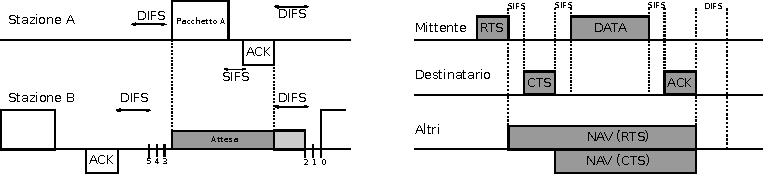
\includegraphics{images/img1.pdf}
	\caption{DCF con metodo accesso base (sinistra) e RTS/CTS (destra)}
	\label{fig:dcfex}
\end{figure}

%\section{Performance analysis of the IEEE 802.11 distributed coordination function}
\section{Analisi della performance IEEE 802.11 DCF}
Uno dei primi e pi\`u rilevanti studi sulle prestazioni del meccanismo DCF \'e quello svolto da Bianchi \cite{bianchi2000performance} che propone la valutazione analitica del saturation throughput, ovvero il limite del throughput di sistema raggiunto all'aumentare del carico sul sistema stesso.
L'analisi \'e stata effettuata con un numero fissato di stazioni ed uno stato di saturazione, ovvero assumendo che ogni stazione abbia sempre un pacchetto disponibile ad essere trasmesso.
Diviso in due parti, lo studio improntato da Bianchi si concentra prima nel fornire una rappresentazione in catena di Markov del comportamento della singola stazione per ottenere la probabilit\`a stazionaria $\tau$ che essa trasmetta un pacchetto in uno slot di tempo casuale.
L'approccio utilizzato fornisce una probabilit\`a indipendente dal tipo di meccanismo di accesso (base o RTS/CTS).
Dopo aver trovato questo valore, analizzando i possibili eventi che possono accadere in un determinato slot temporale, lo studio si conclude esprimendo il throughput dei due possibili metodi di accesso al mezzo trasmissivo in funzione del valore $\tau$.

$$
\begin{cases}
  P \{ i, k| i, k + 1\}  =1 	 &\qquad k \in (0, W_{i}-2) \ i \in (0,m) \\ 
  P \{ 0, k| i, 0\}  =(1-p)/W_{0} 	 &\qquad k \in (0, W_{0}-1) \ i \in (0,m) \\ 
  P \{ i, k| i-1, 0\}  =p/W_{i} 	 &\qquad k \in (0, W_{i}-1) \ i \in (1,m) \\ 
  P \{ m, k| m, 0\}  =p/W_{m} 	 &\qquad k \in (0, W_{m}-1) \\
\end{cases}
$$

La prima equazione tiene conto del decremento del tempo di backoff all'inizio di ogni slot di tempo mentre la seconda equazione del fatto che un nuovo pacchetto in seguito ad una trasmissione con successo inizia con un backoff stage pari a 0.
I restanti due casi esprimono il sistema in caso di fallimento nella trasmissione.
In particolare la terza equazione esprime come avvenga un aumento del backoff stage e la scelta di un nuovo valore di backoff iniziale nel range (0,W\textsubscript{i}).
Infine, l'ultima equazione, modella il massimo valore m che il tempo di backoff pu\`o assumere.
Dopo aver trovato la formula chiusa della catena di Markov si pu\`o esprimere la probabilit\`a $\tau$ che una stazione trasmetta in uno slot di tempo casuale.
Poich\`e la trasmissione avviene quando il timer di backoff raggiunge lo 0, a prescindere dal backoff stage il valore di tau \'e pari a:


\begin{equation}
\tau = \frac{2(1-2p)}{(1-2p)(W+1)+pW(1-(2p)^m)}
\end{equation}

Il valore di p, ovvero della probabilit\`a di collisione, \'e pari alla probabilit\`a che una delle restanti n-1 stazioni decida di trasmettere un pacchetto.

\begin{equation}
1-(1-\tau)^{n-1}
\end{equation}

Possiamo quindi dire che 

\begin{equation}
\tau(p) = \frac{2}{1+W+pW \sum_{i=0}^{m-1}(2p)^i}
\end{equation}

Per calcolare quindi S, il throughput normalizzato, ovvero il periodo di tempo in cui il canale \'e utilizzato per trasmettere correttamente pacchetti, Bianchi ha poi definito le probabilit\`a degli eventi che possono accadere in uno slot di tempo.
In particolare, viene identificata con P\textsubscript{tr} la probabilit\`a che ci sia almeno una trasmissione nello slot di tempo e, poich\`e ogni stazione trasmette sul canale con probabilit\`a $\tau$, si ha:

\begin{equation}
P_{tr} = 1-(1-\tau)^n
\end{equation}

La probabilit\`a P\textsubscript{s} che una trasmissione avvenga correttamente \'e quindi data dalla probabilit\`a che esattamente una stazione trasmetta condizionata dalla probabilit\`a che almeno una stazione trasmetta.

\begin{equation}
P_{s} = \frac{n\tau(1-\tau)^{n-1}}{P_{tr}} = \frac{n\tau(1-\tau)^{n-1}}{ 1-(1-\tau)^n}
\end{equation} 

Si pu\`o ora descrivere S come il rapporto

\begin{equation}
S = \frac{E[payload \ trasmesso \ in \ uno \ slot \ di \ tempo]}{E[lunghezza \ dello \ slot \ di \ tempo]}
\end{equation}

Dato che E[P] e' la dimensione media di un pacchetto, la media di informazione trasmessa correttamente in uno slot di tempo e' pari a $P_{tr}P_{s}E[P]$, poich\`e una trasmissione corretta avviene in uno slot con probabilit\`a $P_{tr}P_{s}$.
Con probabilit\`a $1-P_{tr}$ lo slot di tempo \'e vuoto, con probabilit\`a $P_{tr}P{s}$ contiene una trasmissione con successo e con probabilit\`a $P_{tr}(1-P_{s})$ una collisione.
L'equazione per ottenere S diventa quindi
\begin{equation}
S = \frac{P_{s} P_{tr} E[P]}{	(1-P_{tr})\sigma + P_{tr} P\textsubscript{s} T_{s} + P_{tr}(1-P_{s})T_{c}}
\end{equation}

In questa equazione si identifica il tempo medio in cui il canale viene visto come occupato per via di una trasmissione avvenuta con successo con $T_{s}$ ed il tempo medio in cui il canale viene visto come occupato per via di una trasmissione con collisione con $T_{c}$.
Questi valori, necessari per il calcolo del throughput, dipendono dal tipo di meccanismo di accesso utilizzato.
Per quanto riguarda il meccanismo di accesso base, identificando con H=$ PHY_{hdr}$ + $MAC_{hdr}$, $\delta$ il ritardo di propagazione e E[P*] la lunghezza media del pi\`u grande pacchetto coinvolto in una collisione:

$$
\begin{cases}
T_{s}^{bas} &= H + E[P] + SIFS + \delta + ACK + DIFS + \delta \\
T_{c}^{bas} &= H + E[P*] + DIFS + \delta \\
\end{cases}
$$

Per il meccanismo di accesso basato su RTS/CTS i valori sono invece

$$
\begin{cases}
\!\begin{aligned}
T_{s}^{rts} =  &\ RTS + SIFS + \delta + CTS + SIFS + \delta + H + E[P]  \\ & + SIFS + \delta + ACK + DIFS + \delta 
\end{aligned}
\\
T_{c}^{rts} = RTS + DIFS + \delta \\
\end{cases}
$$

Il modello presentato da Bianchi si \'e rivelato, dopo validazione tramite simulazione, efficace per rappresentare i diversi schemi di accesso utilizzati da DCF: in particolare quello base, RTS/CTS ed una combinazione dei due che non \'e stata riportata.
I risultati ottenuti dal modello mostrano che la performance del metodo di accesso base dipende fortemente sui parametri del sistema, principalmente il numero di stazioni connessi ed i parametri minimi della finestra di contesa.
Questi ultimi sono per\`o meno influenti sul metodo RTS/CTS che si presenta come la migliore opzione di accesso al metodo per reti di grandi dimensioni per via della possibilit\`a di arginare il problema dei terminali nascosti ed un minore tempo impiegato durante la collisione quando pi\`u stazioni trasmettono contemporaneamente.

\newpage

\section{TCP e DCF, analisi della performance }

Lo studio condotto da Wu et al \cite{wu2002performance} propone un modello basato su quello di Bianchi che tiene per\`o conto del limite di tentativi di ritrasmissione di un frame.
In aggiunta, viene proposto un miglioramento allo standard 802.11 con l'introduzione di DCF+.
Questo meccanismo di accesso al metodo di trasmessione \'e introdotto per cercare di sopperire alle problematiche di performance di cui protocolli di livello trasporto soffrono in reti wireless \cite{xylomenos1999tcp}.
In particolare, lo studio si concentra sul risolvere la contesa per il canale di trasmissione che avviene durante lo scambio di dati ed ACK TCP, meccanismo che potrebbe causare collisioni e un degrado delle prestazioni.
La soluzione proposta \'e inoltre compatibile con DCF definito dallo standard 802.11, questo vuol dire che in una stessa rete possono coesistere e comunicare stazioni che supportano due metodi di accesso al mezzo trasmissivo diversi.

Il principale cambiamento che DCF+ apporta \'e quello di utilizzare il MAC ACK specificato nello standard 802.11 come un RTS.
Questo \'e in linea con l'implementazione di DCF che prevede l'invio di un ACK in caso di una trasmissione ricevuta con succeso e permette una retrocompatibilit\`a con stazioni che non implementano DCF+.

In figura si mostra un esempio del funzionamento di DCF+ assumendo che la stazione destinatario debba, oltre a ricevere un frame dal mittente, anche inviargli un pacchetto dati.
Successivamente alla corretta ricezione del frame dati il destinatario procede ad inviare un ACK al mittente che, come gi\`a introdotto, viene considerato come un RTS ed utilizzato per inizializzare anche il NAV delle altre stazioni in ascolto. 
Come da implementazione del DCF il mittente risponde a questo frame con un CTS ed inizializza i valori del NAV pari alla lunghezza del frame di dati che deve ricevere.
L'operazione si conclude con l'invio del pacchetto ed un normale ACK di riscontro.
Per quanto riguarda il metodo di accesso RTS/CTS la procedura differisce solo per l'aggiunta dei due pacchetti iniziali che permettono alle stazioni di impossessarsi del mezzo trasmissivo.

\begin{figure}[!htb]
	\centering
	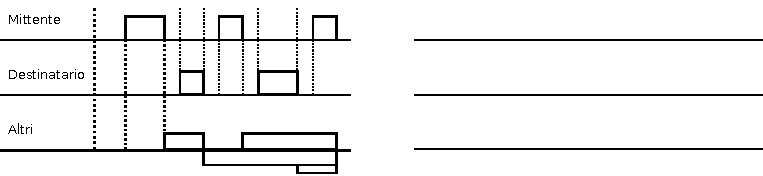
\includegraphics{images/img2.pdf}
	\caption{DCF+ con metodo accesso base (sinistra) e RTS/CTS (destra)}
	\label{fig:dcf+ex}
\end{figure}

Il funzionamento di DCF+ come presentato si basa, per\`o, su due assunzioni:

\begin{itemize}
	\item La stazione mittente che riceve l'ACK sia in grado di determinare, in base al campo della durata presente nel frame, se il destinatario ha un pacchetto dati pronto per l'invio.
	\item Le stazioni, tramite campi nel frame dati e record locali, siano in 		grado di determinare se il destinatario supporti DCF+.
\end{itemize}

Il modello utilizzato da Wu et al per l'analisi di questo metodo di accesso si basa su una estensione del modello proposto da Bianchi.
In particolare, a parit\`a di assunzioni, viene proposta una catena di Markov in cui vengono considerati gli effetti del limite di ritrasmissioni di frame:

$$
\begin{cases}
  P \{ i, k| i, k + 1\}  =1 	 &\qquad k \in (0, W_{i}-2) \ i \in (0,m) \\ 
  P \{ 0, k| i, 0\}  =(1-p)/W_{0} 	 &\qquad k \in (0, W_{0}-1) \ i \in (0,m) \\ 
  P \{ i, k| i-1, 0\}  =p/W_{i} 	 &\qquad k \in (0, W_{i}-1) \ i \in (1,m) \\ 
  P \{ 0, k| m, 0\}  =p/W_{0} 	 &\qquad k \in (0, W_{m}-1) \\
\end{cases}
$$

%b0,0

Questa differenza si ripercuote anche sui valori di $\tau$ e $p$.
In aggiunta, poich\`e viene considerato anche l'effetto timeout dell'ACK, il modello differir\`a da quello proposto da Bianchi anche nei valori di $T^{bas}$ e $T^{rts}$ che saranno, rispettivamente:

$$
\begin{cases}
T_{s}^{bas} &= H + E[P] + SIFS + \delta + ACK + DIFS + \delta \\
T_{c}^{bas} &= DIFS + H + E[P*] + SIFS + ACK \\
\end{cases}
$$

$$
\begin{cases}
\!\begin{aligned}
T_{s}^{rts} =  &\ RTS + SIFS + \delta + CTS + SIFS + \delta + H + E[P]  \\ & + SIFS + \delta + ACK + DIFS + \delta 
\end{aligned}
\\
T_{c}^{rts} = DIFS + RTS + SIFS + CTS \\
\end{cases}
$$

Il modello analitico sviluppato da questo studio si \'e dimostrato pi\`u accurato rispetto a quello proposto da \cite{bianchi2000performance} in seguito alle simulazioni svolte.
Quest ultimo infatti sovrastima il throughput poich\`e non considera il limite di ritrasmissioni ed il timeout dovuto all'ACK.
Le prestazioni di DCF+ sono poi state comparate a quelle di DCF utilizzando il modello presentato, evidenziando un miglioramento in metriche quali: goodput, fairness nell'utilizzo del mezzo trasmissivo e delay a livello MAC.

\newpage
\section{IEEE 802.11E EDCF}
Fino allo standard IEEE 802.11e \cite{ieee05} il modello della WLAN pu\`o essere visto come una versione wireless di Ethernet che supporta un servizio best effort.
L'aumento dei servizi offerti in streaming e VoIP ha per\`o reso necessaria l'implementazione di meccanismi per il supporto quality of service (QoS), ovvero la possibilit\a` di fornire una diversa priorit\`a a diverse applicazioni o utenti.
Nel principio 802.11 non fornisce questo supporto di differenziare frame in base a priorit\`a, tutto ci\`o che fornisce DCF \'e un accesso al canale in contesa con uguale probabilit\`a per tutte le stazioni.
Lo standard 802.11e definisce due miglioramenti al fine di supportare QoS mediamente l'introduzione di Enhanced Distributed Coordination Function (EDCF) e Hybrid Coordination Function (HCF).
In EDCF vengono implementate delle categorie di traffico (TC) a cui vengono associate diverse priorit\`a come mostrato nella tabella \ref{table:catvalues}.

%\begin{flushright}
\begin{table}[h]
%\centering
\begin{tabular}{| l | l | l | l |}
	\hline 
	Priorit\`a  & 802.1D & Categoria & Descrizione \\ \hline
	Bassa & 1 & AC\textunderscore BK & Background \\ \hline
     & 2 & AC\textunderscore BK & Background \\ \hline
	 & 0 & AC\textunderscore BE & Best Effort \\ \hline
	 & 3 & AC\textunderscore BK & Best Effort \\ \hline
	 & 4 & AC\textunderscore VI & Video \\ \hline
	 & 5 & AC\textunderscore VI & Video \\ \hline
	 & 6 & AC\textunderscore VO & Voce \\ \hline
	Alta & 7 & AC\textunderscore VO & Voce \\ \hline
\end{tabular}
%\end{flushright}
\centering
\caption{Tabella categorie accesso}
\label{table:catvalues}
\end{table}

I frame delle stazioni vengono quindi divisi in diverse istanze di backoff, ognuna con dei parametri specifici alla categoria di traffico \ref{fig:edcf}.
Nel periodo di contesa per il mezzo trasmissivo, ogni categoria di traffico cerca di accedere ad una transmission opportunity (TXOP) ed inizia un periodo di backoff indipendente dopo che il canale \'e inattivo per almeno un Arbitration Interframe Space (AIFS).
Se durante il periodo di backoff il canale torna ad essere utilizzato, come per DCF, EDCF aspetta che il canale torni ad essere libero prima di diminuire il valore di backoff.
Per via delle categorie di traffico, una singola stazione pu\`o implementare fino ad otto code interne realizzate come stazioni virtuali.
Se pi\`u di una stazione raggiunge il valore 0 nel backoff, uno scheduler ha il compito di evitare una collisione tra le due stazioni virtuali dando la TXOP alla stazione con priorit\`a pi\`u alta.

\begin{figure}[!htb]
	\centering
	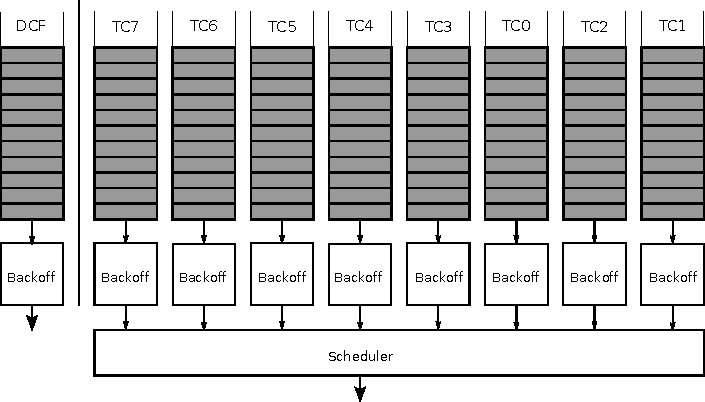
\includegraphics{images/img3.pdf}
	\caption{DCF (sinistra) e EDCF con otto backoff virtuali (destra)}
	\label{fig:edcf}
\end{figure}

Durante l'intervallo TXOP, definito da un tempo di inizio ed una massima durata, una stazione ha il diritto di trasmettere sul canale.
L'intervallo TXOP viene allocato tramite una contesa (EDCF-TXOP) o assegnato attraverso HCF (polled-TXOP).
La durata dell'intervallo \'e definita dai beacon frames dell'AP per quanto riguarda EDCF-TXOP e specificato nel frame del poll per quanto riguarda HCF.

Diversi studi sono stati improntati sulla performance di EDCF, in particolare \cite{mangold2002ieee} dopo aver simulato l'uso di EDCF ne evidenzia una soluzione efficiente per l'implementazione QoS su reti WLAN e la retrocompatibilit\`a con stazioni che non implementano questo metodo di accesso.
Con l'opportuna scelta di parametri, stazioni EDCF riescono infatti ad avere priorit\`a sul canale rispetto a stazioni che implementano DCF.

Xiao \cite{xiao2004performance} ha successivamente fornito un modello analitico, seguendo le orme di Bianchi, di EDCF.
Utilizzando metriche di backoff quali: dimensione iniziale della finestra, limite di ritrasmissioni e il fattore di incremento della finestra di backoff i risultati ottenuti dallo studio mostrano come una categoria di traffico possa rubare banda ad un altra categoria in caso questa aumenti il valore delle suddette metriche.
In aggiunta, viene suggerita una ridimensione del limite di ritrasmissioni per traffico di tipo video per aumentare throughput e migliorare il delay.

\newpage


\section{IEEE 802.11N e 802.11AC}

Attualmente la maggior parte dei router in commercio ed utilizzati in reti locali sono conformi allo standard 802.11n ed, in particolare, a quello 802.11ac.
Il primo, con l'obiettivo di aumentare il throughput degli standard precedenti, fornisce supporto per frame aggregation e multiple-input and multiple-output (MIMO).
Come suggerisce il nome, il frame aggregation permette ad un trasmettitore di inviare pi\`u di un frame in una singola trasmissione.
Questa funzionalita, come studiato da  \cite{skordoulis2008ieee}, si rivela molto efficace per l'aumento del throughput della rete e per la riduzione del ritardo di trasmissione.
La tecnologia MIMO fa utilizzo di una moltitudine di antenne in ricezione ed invio per trasmettere simultaneamente pi\`u stream di dati utilizzando propagazione a pi\`u vie.
Il successivo standard 802.11ac, utilizzato maggiormente nella realizzazione del tirocinio, estende MIMO per permettere un uso multi utente, chiamato  MU-MIMO.

\section{Radiotap}

Un header radiotap \'e un meccanismo che viene utilizzato per aggiungere informazioni ad un frame 802.11 al momento della sua cattura.
Pur non facendo parte in alcun modo di pacchetti 802.11 l'importanza delle metriche fornite ed il supporto ai pi\`u utilizzati sistemi operativi lo rendono 
uno standard per la ricezione di frame 802.11.
L'header radiotap viene aggiunto al frame catturato dal device di rete, o dal suo driver, e contiene quindi informazioni fornite dalla particolare stazione che riceve e non di quella che trasmette.

Si elencano ora alcuni dei campi presenti nel radiotap header, in particolare quelli utilizzati per lo sviluppo della soluzione proposta dal tirocinio:

\begin{itemize}
	\item Antenna: antenna in ricezione o tramissione utilizzata per il pacchetto.
	\item Channel: frequenza del canale utilizzato per trasmettere il pacchetto.
	\item Antenna Signal: potenza del segnale in ricezione all'antenna.
	\item Antenna Noise: rumore di sottofondo in ricezione all'antenna.
	\item Timestamp: l'istante di tempo in cui \'e stato ricevuto il pacchetto.
\end{itemize}

In particolare con l'uso di queste metriche, oltre ad identificare su quale canale un AP stia utilizzando per le proprie trasmissioni, si pu\`o fornire un valore riguardante la bont\`a del segnale Wi-Fi.

La differenza tra antenna signal ed antenna noise fornisce, infatti, un parametro chiamato Signal-to-Noise-Ratio (SNR) che viene per classificare la qualit\`a del segnale.
In generale i valori del SNR si possono cos\`i catalogare:

\begin{itemize}
	\item >40dB: segnale eccellente, massima velocit\`a.
	\item 25db-40db: segnale molto buono, ottima velocit\`a.
	\item 15db-25db: segnale basso, buona velocit\`a.
	\item 10db-15db: segnale molto basso, bassa velocit\`a.
	\item 5db-10db: nessun segnale.
\end{itemize}

Avere un SNR accettabile per ogni dispositivo connesso alla rete \'e fondamentale per la performance generale, poich\`e uno scarso segnale contribuisce fortemente all'aumentare del numero di ritrasmissioni e quindi una diminuzione del throughput del sistema Wi-Fi.

\section{Software di monitoraggio Wi-Fi}

I metodi di accesso al mezzo trasmissivo e le metriche per misurare la bont\`a del segnale presentati in questo capitolo sono alla base del funzionamento dei software pi\`u utilizzati per il monitoraggio di reti Wi-Fi.
%Software a pagamento
%Software manufacturer bounded
%Progetti abbandonati
La soluzione open-source pi\`u utilizzata e sviluppata \'e sicuramente la gi\`a menzionata Kismet, che tra le tante funzionalit\`a permette, tramite API, la visualizzazione di tutti i dispositivi connessi ad un access point e ne fornisce eventuali valori del segnale.
Questo tipo di approccio non permette per\`o una visione di insieme della topologia Wi-Fi poich\`e, ad esempio, l'individuazione di eventuali repeater non \'e automatizzata.

Funzioni simili a quelle di Kismet si possono trovare nel prodotto UniFi \cite{unifi} di Ubiquity che fornisce una panoramica dettagliata dell'attivit\`a di rete e degli indici di connessione dei dispositivi.
Purtroppo, software di questo tipo sono generalmente proprietari e limitati ad un utilizzo con dispositivi specifici del produttore.
Questo tipo di soluzione non \'e quindi ottimale per la gestione di una rete locale domestica dove i dispositivi connessi sono generalmente di diversi produttori e non di livello professionale.

Pi\`u comuni sono software come NetSpot \cite{netspot}, Kismac e inSSIder \cite{inssider} che forniscono invece una visione della rete Wi-Fi limitata agli access point presenti nelle vicinanze.
In questo modo \'e possibile identificare eventuali problemi di connessione Wi-Fi dovuti alla sovrapposizione di pi\`u reti WLAN sullo stesso canale.

\chapter{Soluzione proposta}
In questo capitolo viene presentata la soluzione proposta per la rilevazione di disservizi nella connettivit\`a di reti locali.
Si analizza brevemente l'architettura del software sviluppato per poi fornirne una descrizione dettagliata della sua implementazione e del software utilizzato nello sviluppo.

\section{Architettura}
L'architettura della soluzione proposta \'e principalmente suddivisa in due parti come mostrato in figura \ref{fig:solproposta}: %FIGURA
\begin{itemize}

\item una libreria che implementa un'operazione di ARP \cite{rfc826} scan, utilizzata per fornire una metrica del round-trip time (RTT) ed associare ad indirizzi IPv4 nella rete locale i rispettivi indirizzi MAC.
Bench\`e l'utilizzo di questa libreria sia facoltativo, nei capitoli successivi si mostrer\`a come i risultati ottenuti dall'operazione di ARP scan migliorino l'accuratezza della ricostruzione della topologia Wi-Fi.
\item una libreria che, dopo aver catturato pacchetti di traffico di rete ed ottenuto i risultati dell' ARP scan, analizza i frame ricevuti e li utilizza per ricostruire una topologia della rete Wi-Fi fornendo valori di bont\`a del segnale.
Questa libreria \'e in grado di ricostruire topologie di reti sia in modalit\`a di cattura attiva o da file di cattura.
\end{itemize}

Le operazioni di cattura di pacchetti in entrambe le librerie sviluppate sono effettuate utilizzando l'API Pcap \cite{pcap}.
In particolare, nella libreria di ARP scanning vengono catturati frame di tipo Ethernet II mentre nella libreria per la ricostruzione della topologia di una rete i frame catturati sono di tipo 802.11.
%Perche'

\begin{figure}[!htb]
	\centering
	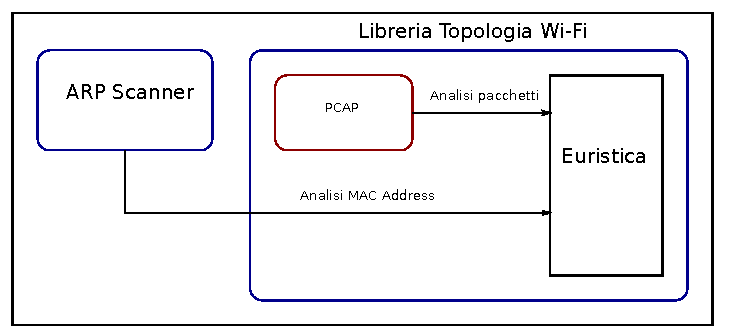
\includegraphics{images/img4.pdf}
	\caption{Architettura soluzione proposta}
	\label{fig:solproposta}
\end{figure}


\section{Implementazione}
Si presentano brevemente, prima dei dettagli implementativi della libreria per la ricostruzione topologica della rete, il funzionamento della libreria utilizzata per la cattura dei pacchetti Pcap e quella implementata per effettuare ARP scanning.

Le librerie sono state sviluppate utilizzando il linguaggio di programmazione C++, un linguaggio nato come miglioramento del C, che permette l'uso del paradigma ad oggetti ed il controllo dell'utente della gestione della memoria.
 %questo ha permesso di combinare l'uso di costrutti ad alto livello come gli oggetti e l'accesso ai frame catturati tramite puntatori.

\subsection{Pcap}

Sviluppata da Tcpdump, libpcap  \'e una libreria scritta in linguaggio C che permette la cattura ed il filtraggio di pacchetti di rete.
La scelta di questa libreria si \'e basata su tre principali aspetti:
\begin{itemize}
	\item Facilit\`a d'uso: libpcap offre astrazioni ad alto livello per la cattura ed il filtraggio di pacchetti di rete.
	\item Filtraggio dei pacchetti: mediante la compilazione di un filter, \'e possibile catturare solo i pacchetti di rete di interesse per l'applicazione.  
	\item Compatibilit\`a: la libreria, oltre ad essere disponibile per la maggior parte dei sistemi operativi moderni, presenta numerosi wrapper per essere integrata in linguaggi di programmazione diversi dal C.
\end{itemize}
Di seguito si descrivono i passi necessari ad effettuare una cattura utilizzando libpcap:
\begin{enumerate}
	\item Scelta dell'interfaccia da utilizzare per la cattura.
	\item Inizializzazione dell'interfaccia e dei parametri della sessione.
	\item Creazione e compilazione del filtro da utilizzare per catturare i pacchetti desiderati. 
	\item Ciclo di ascolto in cui vengono analizzati, uno ad uno, i pacchetti catturati.
	\item Chiusura della sessione di cattura.
\end{enumerate}

%\newpage

\subsection{ARP Scan}

La libreria di ARP scan sviluppata permette la scoperta di tutti i dispositivi all'interno della rete locale.
Questa operazione viene effettuata inviando un numero di pacchetti ARP ad ogni possibile indirizzo IPv4 presente nella sottorete per poi, utilizzando libpcap, riceverne eventuali riscontri.

Il risultato ottenuto \'e un'associazione tra indirizzo IP ed indirizzo media access control (MAC), un indirizzo fisico univoco assegnato ad ogni scheda di rete dal proprio produttore.
L'indirizzo MAC cos\`i ottenuto verr\`a poi utilizzato per fornire una maggiore accuratezza nella ricostruzione della topologia Wi-Fi della rete locale in esame.

Sebbene questo sia il motivo principale di implementazione della libreria, \'e inoltre possibile ricavare una misura del round-trip time verso ogni dispositivo connesso alla rete, in modo analogo al ping attraverso richieste ICMP.
A differenza di quest'ultimo che pu\`o essere ignorato da alcuni tipi di dispositivi, utilizzando l'ARP ping con un numero di pacchetti appropriato \'e possibile ricevere riscontro da tutti i dispositivi attualmente connessi alla rete locale.
In particolare, i dispositivi che tendono ad ignorare questo tipo di richieste sono quelli di tipo mobile come smartphone e tablet nei momenti di non utilizzo da parte dell'utente.

Bench\`e ci siano gi\`a diverse implementazioni funzionanti per i sistemi operativi pi\`u utilizzati, si \'e deciso di sviluppare una libreria basilare che svolga solo le operazioni necessarie per la ricostruzione topologica della rete.
Si \'e cercato  in questo modo di limitare l'utilizzo di risorse e fornire una soluzione la cui implementazione \'e indipendente dal sistema operativo e basata solamente sull'uso di libpcap.

\newpage

%La libreria \'e stata scritta utilizzando il linguaggio di programmazione C++  

%ARP
%Pcap
%monitor mode, svantaggi
%Tipi di messaggi che filtriamo
%MAC header
%Tipi op e tipi header
%Euristica

%ascolto Attivo / ascolto passivo
\subsection{WiFi-Topology}
Dopo aver introdotto nelle sezioni precedenti una vista dell'architettura, purch\`e basilare, e le librerie fondamentali per il funzionamento della soluzione proposta si discute ora l'implementazione della principale libreria sviluppata durante il tirocinio.

La ricostruzione della topologia Wi-Fi delle reti viene effettuata attraverso l'analisi del traffico originato dalle stazioni presenti nelle vicinanze del dispositivo su cui il software \'e in esecuzione.

Questo tipo di cattura, come descritto precedemente, \'e effettuata utilizzando la libreria libpcap che permette di utilizzare un'interfaccia di tipo Wi-Fi in una particolare modalit\`a, chiamata monitor mode, di cui si espone di seguito il funzionamento.

\subsubsection{Monitor mode}
La cattura in monitor mode, o RFMON (Radio Frequency MONitor), permette ad una interfaccia di rete wireless di catturare tutto il traffico passante per un canale Wi-Fi.

In questa modalit\`a una scheda di rete non \'e associata ad alcun access point o rete ad-hoc e si pone in uno stato di ascolto in maniera completamente trasparente ad altri dispositivi wireless presenti nelle vicinanze.
Per effettuare ci\`o non vengono rispettati i normali comportamenti di una stazione operante con il protocollo 802.11, come ad esempio l'invio di ACK descritto nel secondo capitolo.
Di conseguenza, in questa modalit\`a, il dispositivo perde la possibilit\`a di trasmettere dati ed il suo utilizzo \'e ristretto ad un singolo canale wireless.
Un'altra limitazione in questo tipo di cattura riguarda il mancato controllo di errori nei pacchetti catturati, effettuato normalmente con un controllo di ridondanza ciclico (CRC).

Nonostante gli svantaggi elencati, questo tipo di modalit\`a trova molto utilizzo nella progrettazione di reti wireless, ad esempio per la scelta di un canale poco utilizzato al fine di diminuire interferenze tra stazioni, o nel cracking di reti protette con WEP .

Nello sviluppo della libreria questa modalit\`a \'e stata utilizzata per catturare diversi tipi di frame 802.11 trasmessi dai dispositivi nelle vicinanze.
Analizzando questo tipo di dati ed i valori di potenze di segnale forniti dal radiotap header \'e stato poi sviluppato un algoritmo per la ricostruzione della topologia delle reti Wi-Fi.
Per fornire una corretta analisi il controllo di ridondanza ciclico per i frame ricevuti  \'e stato integrato nella libreria sviluppata, in modo da poter evitare eventuali incoerenze tra la topologia ricostruita e quella effettiva.
In aggiunta, poich\`e la modalit\`a monitor dissocia la scheda di rete da un access point e cattura tutto il traffico passante per un canale, la libreria sviluppata non si limita a ricostruire una particolare rete di cui si \'e interessati ma fornisce una visione di tutte quelle nelle vicinanze.
Per sopperire all'impossibilit\`a di ascoltare su pi\`u di un canale si \'e fatto uso di uno script per effettuare channel hopping, in modo da poter catturare traffico per qualche secondo su ciascun canale.

Il compromesso principale dell'uso della monitor mode resta quello di dover dedicare completamente un'interfaccia Wi-Fi alla cattura dei frame dissociandola dalla rete locale che si vuole monitorare.
Per questo motivo, su dispositivi dotati di una sola scheda di rete, non \'e possibile mantenere costantemente attiva la cattura perdendo quindi la possibilit\`a di assistere a cambi nella topologia di rete in tempo reale. 
Un recente studio \cite{zanetti2010non} ha evidenziato come sia possibile virtualizzare, senza perdita di prestazioni, interfacce per la cattura di traffico in modalit\`a promiscua o, come in questo caso, in monitor mode.

Nella prossime sezioni vengono introdotti in dettaglio i frame catturati in questa modalit\`a e come essi sono utilizzati per la ricostruzione della topologia della rete.

\subsubsection{MAC Frame}

Prima di mostrare come avviene l'analisi del traffico si introduce la struttura generale dei frame catturati tramite monitor mode ed i tipi rilevanti al funzionamento della libreria.
Nei protocolli di rete wireless 802.11 un MAC frame, rappresentato in figura \ref{fig:macframe}, \'e composto da campi comuni a tutti i tipi di frame e da campi specifici ad alcuni di essi.

\begin{figure}[!htb]
	\centering
	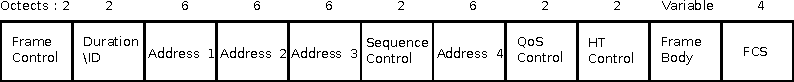
\includegraphics{images/img5.pdf}
	\caption{MAC frame}
	\label{fig:macframe}
\end{figure}

Un frame 802.11 contiene quindi un MAC header di lunghezza pari a 34 byte, un body di lunghezza variabile in base al tipo di frame catturato ed infine un campo di 4 byte per il controllo degli errori.

Di seguito si fornisce una breve descrizione di tutti i campi presenti nel MAC header, in particolare di quelli utilizzati durante l'implementazione della libreria:

\newpage

\begin{itemize}
	\item Frame Control: 2 byte che forniscono informazioni sul tipo del frame.
	\item Duration/ID: 2 byte che indicano alle stazioni la durata della trasmessione e viene usato per inizializzare il valore del NAV introdotto nel secondo capitolo.
	\item Address 1-2-3-4: 6 ottetti che identificano unicamente un dispositivo tramite   indirizzo MAC.
	\item Sequence Control: diviso in due campi di 12 e 4 bit che indicano, rispettivamente, il numero di sequenza ed il numero del frammento del pacchetto.
	\item QoS Control: 2 byte che identificano i parametri QoS in un frame di dati.
	\item HT Control: 2 byte aggiunti dallo standard 802.11n.
	\item Frame Body: campo di lunghezza e tipo variabile, payload del frame.
	\item FCS: 4 byte di frame check sequence, un codice di rilevazione di errore.
\end{itemize}

I campi interessanti per la ricostruzione della topologia di una rete includono il frame control, gli indirizzi MAC, il body del frame ed il FCS.
In particolare, nella figura \ref{fig:framecontrolfields}, possiamo osservare come il frame control sia suddiviso in 11 sottocampi.

\begin{figure}[!htb]
	\centering
	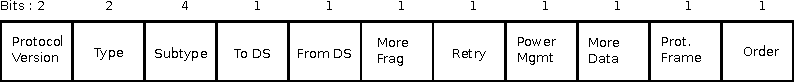
\includegraphics{images/img6.pdf}
	\caption{Frame Control Fields}
	\label{fig:framecontrolfields}
\end{figure}

Il primo campo, protocol version, indica la versione del protocollo 802.11 in uso dal frame ed \'e sempre pari a 0 poich\`e attualmente esiste una sola versione di questo protocollo.

Il secondo e terzo campo del frame control indicano invece il tipo e sottotipo del frame ricevuto.Questo tipo di informazione \'e fondamentale per una corretta analisi poich\`e a diversi tipi e sottotipi di frame corrispondono diversi campi nel frame body.

Data la lunghezza pari a 2 bit, un frame nello standard 802.11 pu\`o essere suddiviso in quattro categorie di tipo diverse, che a loro volta possono contenere sedici sottocategorie codificate con 4 bit:
\begin{itemize}
	\item 00- Management Frame: forniscono informazioni sullo stato della rete e sono utilizzati per la connessione e disconnessione di dispositivi.
	\item 01- Control Frame: assistono la trasmissione di data frame e per amministrare l'accesso al mezzo al mezzo trasmissivo.
	\item 10- Data Frame: contengono dati di protocolli di livello superiore all'interno del loro body.
	\item 11- Reserved: tipo di frame riservato e non utilizzato nello standard 802.11.
\end{itemize}

L'utilizzo e il tipo di analisi effettuata su questi tipi di frame ed i loro sottotipi verr\`a introdotto in apposite sezioni.

I successivi due campi del frame control, To DS e From DS, sono di particolare importanza per lo studio effettuato sulla ricostruzione della topologia di rete.
Questi due bit possono essere utilizzati per determinare quando un frame \'e immesso nel mezzo trasmissivo wireless e quando, invece, ne esce.

Di seguito si evidenziano i possibili valori di verit\`a dei due campi:

\begin{itemize}
	\item To DS=0, From DS=0 : il frame non deve lasciare il mezzo trasmissivo, valore generalmente associato a tipi di frame come: management e control.
	\item To DS=0, From DS=1 : il frame proviene da un access point e sta entrando nel mezzo trasmissivo wireless.
	\item To DS=1, From DS=0 : il frame proviene da un client e sta uscendo dal mezzo trasmissivo wireless.
	\item To DS=1, From DS=1 : il frame \'e destinato ad un'altra rete wireless.
\end{itemize}

Accoppiando questo tipo di analisi del mezzo trasmissivo con i valori di segnale ottenuti tramite Radiotap \'e possibile rilevare anche eventuali dispositivi connessi ad un access point via cavo, purch\`e il traffico analizzato contenga un cambio di mezzo trasmissivo.

Un esempio, che sar\`a discusso anche nel prossimo capitolo, potrebbe essere quello di un router collegato via cavo ad un access point ed un numero di dispositivi connessi in Wi-Fi a quest'ultimo.

\newpage

\subsubsection{MAC Address}

Un MAC address \'e un identificatore unico associato ad un'interfaccia di rete dal proprio costruttore e viene utilizzato nel protocollo 802.11 per l'instradamento dei frame.
L'indirizzo \'e formato da una struttura di 48 bit divisa in 6 ottetti, come mostrato in figura \ref{fig:macaddress}.
%Guidelines for Use of Extended Unique Identifier (EUI), Organizationally Unique Identifier (OUI), and Company ID
Per mantenere l'unicit\`a tutte le schede di rete prodotte \'e stato introdotto uno standard, chiamato EUI-48 e gestito dalla IEEE, che divide l'indirizzo MAC in due parti:
\begin{itemize}
	\item Organisationally Unique Identifier (OUI): identifica unicamente un produttore di schede di rete ed \'e assegnato dalla IEEE.
	\item Network Interface Controller (NIC): identifica unicamente una determinata scheda di rete e viene assegnata dal prodottore.
\end{itemize}

\begin{figure}[!htb]
	\centering
	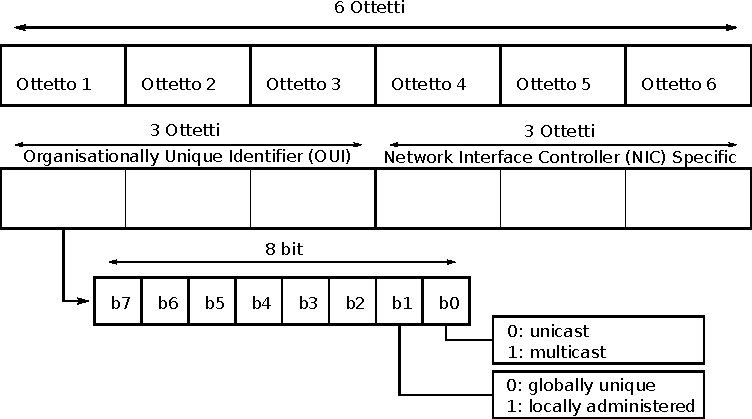
\includegraphics{images/img7.pdf}
	\caption{Mac Address}
	\label{fig:macaddress}
\end{figure}

In aggiunta, un indirizzo MAC pu\`o essere universalmente (UAA) o localmente (LAA) assegnato.
Questa diversificazione viene effettuata attraverso il valore del secondo bit meno signficativo del primo ottetto.
Per quanto riguarda gli indirizzi UAA, questo bit viene posto a 0 ed il valore del primo ottetto \'e pari a quello del OUI.
Al contrario, un valore del bit pari ad 1 identifica un indirizzo LAA che viene generalmente assegnato da eventuali amministratori di rete.

La differenziazione del tipo di trasmissione in unicast e multicast avviene in maniera simile, in questo caso l'identificazione avviene mediante il bit meno significativo del primo ottetto.

Un valore pari a 0 equivale ad una trasmissione unicast mentre un valore pari ad 1 una trasmissione di tipo multicast.
Infine, l'indirizzo di broadcast \'e ottenuto ponendo un valore pari ad 1 ad ogni bit dell'indirizzo MAC.

Come visto precedentemente, un MAC header \'e costituito da quattro indirizzi MAC il cui valore e significato varia in base al tipo di frame ed ai valori To DS e From DS.
Gli indirizzi possono essere dei seguenti tipi:
\begin{itemize}
	\item Receiver Address (RA): indirizzo della stazione che riceve il frame.
	\item Transmitter Address (TA): indirizzo della stazione che trasmette il frame.
	\item Basic Service Set Identifier (BSSID): indirizzo dell'access point della rete.
	\item Destination Address (DA): indirizzo di destinazione finale del frame.
	\item Source Address (SA): indirizzo sorgente del frame.
\end{itemize}

Nella figura \ref{table:addressvalue} si mostrano le varie combinazioni che gli indirizzi MAC possono rappresentare in base ai valori presenti nel frame control.

\begin{table}[h]
\centering
\begin{tabular}{| l | l | l | l | l | l |}
	\hline 
	To DS  & From DS & Address 1 & Address 2 & Address 3 & Address 4\\ \hline
	 0 & 0 & RA=DA & TA=SA & BSSID & N/A \\ \hline
     0 & 1 & RA=DA & TA=BSSID & SA & N/A\\ \hline
	 1 & 0 & RA=BSSID & TA=SA & DA & N/A\\ \hline
	 1 & 1 & RA & TA & DA & SA\\ \hline
\end{tabular}
%\end{flushright}
\centering
\caption{Tabella uso indirizzi MAC }
\label{table:addressvalue}
\end{table}

%Aggiungere ref
%Accennare qui indirizzo locale repeater?

\newpage

\subsubsection{Management Frame}

I frame di tipo management vengono utilizzati dalle stazioni e dall'access point per regolare l'accesso e disconnessione alla rete WLAN.
Questo tipo di frame permette, durante la parte di analisi del traffico, di identificare gli access point  attivi ed eventuali dispositivi che stiano cercando di accedervi.
%Bench\`e i sottotipi definiti per questo tipo di frame siano 16 si elencano, in tabella \ref{table:managementframes}, solo quelli effettivamente utilizzati dalla libreria per la costruzione topologica della rete.

%\begin{table}[h]
\begin{wraptable}{r}{8cm}
\centering
\begin{tabular}{| l | l |}
	\hline
	Subtype  & Descrizione \\ \hline
	%0000 & Association Request \\ \hline
	0001	 & Association Response 	\\ \hline
  %  0010	 & Reassociation Request \\ \hline
	%0011	 & Reassociation Response \\ \hline
	0100	 & Probe Request \\ \hline
	%0101	 & Probe Response \\ \hline
%	0110	& Timing Advertisement \\ \hline
	%0111	& Reserved \\ \hline
	1000 &	Beacon \\ \hline
	%1001	& ATIM \\ \hline
	1010	& Disassociation \\ \hline
	%1011	& Authentication \\ \hline
	1100	& Deauthentication \\ \hline
	%1101	& Action \\ \hline
	%1110	& Action No Ack (NACK) \\ \hline
	%1111	& Reserved \\ \hline 
\end{tabular}
%\end{flushright}
\centering
\caption{Sottotipi Mgmt Frame}
\label{table:managementframes}
%\end{table}
\end{wraptable}

Bench\`e i sottotipi definiti per questo tipo di frame siano 16 si elencano, in tabella \ref{table:managementframes}, solo quelli effettivamente utilizzati dalla libreria per la costruzione topologica della rete.

Il sottotipo di frame pi\`u interessante per questa operazione \'e quello di Beacon, che viene utilizzato dagli access point per annunciare la presenza di una rete WLAN alle stazioni vicine.

Nel frame body sono presenti 5 campi obbligatori:

\begin{itemize}
	\item Timestamp: 8 byte che indicano il tempo di attivit\`a dell'access point.
	\item Beacon Interval: 2 byte che indicano la frequenza di invio di un beacon frame.
	\item Capability Information: 2 byte utilizzati per specificare 
	funzionalit\`a aggiuntive dell'access point.
	\item	SSID: lunghezza variabile, identifica il nome logico di una rete WLAN.
	\item Supported Rates: specifica la velocit\`a in Mbps che la stazione offre.
\end{itemize}

La libreria utilizza il Beacon frame per determinare se il MAC address del mittente sia  un access point che avr\`a, eventualmente, una serie di dispositivi a lui connesso.
In aggiunta, analizzando il radiotap header di un Beacon frame \'e possibile fornire un quadro completo sui dettagli della rete che viene annunciata, in particolare: canale in uso, potenza del segnale.

Come intuibile dalla descrizione, i frame di Association Response, Disassociation e Deauthentication indicano connessioni e disconnessioni di dispositivi alla rete wireless.
In particolare i tipi di frame riguardanti le disconnessioni sono fondamentali per evitare di fornire una topologia della rete in cui vengano identificati come collegati dispositivi che non sono pi\`u appartenenti alla rete.
Nonostante la loro importanza, la frequenza con cui questi frame vengono analizzati dipende fortemente dal tipo di monitoraggio che si effettua: costante o ad istanti di tempo.

A differenza dei frame precedenti il Probe Request viene inviato da un dispositivo che si pone in cerca di reti WLAN a cui accedere e  la sua analisi avviene solo per misurare parametri di bont\`a del segnale poich\`e il dispositivo non \'e connesso a nessuna rete.

\subsubsection{Control Frame}

I frame di tipo control assistono l'invio di frame management e data, amministrando l'accesso al mezzo trasmissivo wireless.

Come evidente dalla tabella \ref{table:controlframes} i principali frame che vengono analizzati corrispondono a quelli introdotti nella presentazione di DCF nel secondo capitolo.
\begin{table}[h]
%\begin{wraptable}{r}{8cm}
\centering
\begin{tabular}{| l | l |}
	\hline
	Subtype  & Descrizione \\ \hline
	1001	 & Block Ack 	\\ \hline
	1011	 & RTS \\ \hline
	1100 &	CTS \\ \hline
	1101	& ACK \\ \hline
\end{tabular}
%\end{flushright}
\centering
\caption{Sottotipi Control Frame}
\label{table:controlframes}
%\end{table}
%\end{wraptable}
\end{table}

In questo tipo di frame, come specificato da DCF, non \'e presente un frame body.
Per questo motivo l'analisi dei control frame da parte della libreria \'e in grado di fornire solamente una relazione di connessione tra due indirizzi MAC e quindi due dispositivi.

\subsubsection{Data Frame}

I Data frame vengono utilizzati nel protocollo 802.11 per la trasmissione di dati provenienti da livelli superiori.

\begin{wraptable}{r}{8cm}
\centering
\begin{tabular}{| l | l |}
	\hline
	Subtype  & Descrizione \\ \hline
	0000	 & Null No Data 	\\ \hline
	0100	 & Data \\ \hline
	1000 &	QoS Data \\ \hline
	1100	& QoS Null No Data \\ \hline
\end{tabular}
%\end{flushright}
\centering
\caption{Sottotipi Data Frame}
\label{table:dataframes}
%\end{table}
\end{wraptable}

In tabella \ref{table:dataframes} si evidenziano i sottotipi di questo frame che vengono analizzati per la ricostruzione della topologia della rete WLAN.

La cattura e l'analisi di questi tipi di frame permette l'identificazione dei dispositivi su cui la trasmissione wireless termina o inizia.

Sfruttando questa informazione \'e quindi possibile identificare per ogni stazione che trasmette un frame il dispositivo a cui esso \'e collegato.

Come verr\`a esposto nella sezione successiva questo procedimento \'e fondamentale per la corretta rappresentazione della topologia di rete e permette di identificare il percorso dei frame inviati da un dispositivo anche in presenza di ripetitori Wi-Fi.

\subsubsection{Analisi ed euristica}

Il funzionamento della libreria pu\`o essere diviso in tre principali fasi delle quali si  spiega, nel dettaglio, il funzionamento:

\begin{enumerate}
	\item Cattura ed analisi dei frame 802.11.
	\item Ispezione degli indirizzi MAC dei dispositivi presenti e di eventuali access point. 
	\item Topologia risultante.
\end{enumerate}

La cattura dei frame 802.11, come precedentemente introdotto, viene effettuata mediante la libreria libpcap ed impostando la scheda di rete Wi-Fi in modalit\`a monitor.
Durante questa procedura, per ogni frame ricevuto dalla scheda di rete, vengono analizzati il radiotap header ed il MAC header.
In particolare, utilizzando il radiotap header, vengono estratte informazioni riguardanti la potenza del segnale della stazione che trasmette il frame ed il canale utilizzato per l'invio.

L'analisi del MAC header \'e cruciale per fornire una corretta ricostruzione della topologia di rete e comprende diversi controlli di correttezza.
In primis viene effettuato un controllo sul FCS per poter scartare tutti i frame corrotti che vengono catturati.
Se il pacchetto ricevuto \'e esente da errori, vengono successivamente analizzati gli indirizzi MAC in base al tipo e sottotipo di frame ricevuto.
In questo controllo vengono scartati tutti pacchetti di tipo data e control i cui indirizzi destinatari sono di tipo broadcast, poich\`e questi tipi di frame non forniscono informazioni su alcun dispositivo connesso.

Soddisfatti questi requisiti gli indirizzi MAC presenti nel frame vengono considerati dispositivi Wi-Fi di interesse e memorizzati per poi poter esser nuovamente ispezionati al termine del procedimento di cattura.

Nel caso in cui il dispositivo analizzato abbia trasmesso almeno un frame di tipo beacon, questo viene considerato come un access point.
\newpage
Per ogni dispositivo, in questo stadio dell'esecuzione, sono quindi noti i seguenti valori:
\begin{itemize}
	\item Canale, potenza e rumore dell'antenna.
	\item Indirizzo MAC.
	\item Lista di indirizzi MAC con cui il dispositivo interagisce.
	\item Nome della rete annunciata (se AP).
\end{itemize}

La fase successiva necessaria per la ricostruzione della topologia di rete consiste nell'associare eventuali indirizzi MAC virtuali e multicast ai rispettivi indirizzi globalmente assegnati.
Questo procedimento \'e necessario per evitare di includere nella topologia Wi-Fi indirizzi MAC che, in realt\`a, non appartengono a nessun dispositivo.
Non \'e affatto raro, infatti, l'utilizzo di indirizzi virtuali da parte di repeater ed access point per la trasmissione in rete o l'uso di multicast da parte di router per l'invio di frame a singoli dispositivi.
Il risultato ottenuto \'e un diretto collegamento tra un indirizzo virtuale al suo indirizzo globalmente assegnato, sia esso ottenuto mediante una precedente ARP scan o dalla cattura di frame 802.11.

Il passo successivo effettuato dalla libreria \'e quello di applicare un'euristica in grado di determinare se un dispositivo di rete abbia pi\`u di una antenna Wi-Fi ed in che modo queste vengano utilizzate.
Gli attuali access point presenti in commercio aderiscono allo standard 802.11AC e sono quindi provvisti di una moltitudine di antenne wireless.
Dopo lo studio di numerosi dispositivi di questo tipo si \'e formulata un'euristica coerente con i comportamenti osservati, basata sulla divisione dell'indirizzo MAC in due sezioni:la prima comprendente i primi cinque ottetti e la seconda il restante ottetto.
Infatti, gli indirizzi MAC delle varie antenne presenti in questo tipo di dispositivi sembrano essere sempre maggiori in valore rispetto all'indirizzo fornito dal produttore.
Considerando quindi tutti gli indirizzi MAC ottenuti dalla cattura di frame ed, eventualmente, anche dall'ARP scan si seleziona quello che presenta un valore minore nell'ultimo ottetto come l'indirizzo effettivo del dispositivo.

L'euristica presentata, in aggiunta a quella implementata per assegnare un indirizzo MAC globale ad uno localmente assegnato, risolve inoltre un altro problema emerso durante lo sviluppo della libreria riguardante l'utilizzo di indirizzi MAC da parte di repeater Wi-Fi.
Durante lo studio approntato sono stati infatti individuati due metodi di funzionamento dei repeater, anche in dispositivi la cui unica differenza risiedeva nel firmware installato.

Uno dei metodi in cui i repeater trattano il traffico \'e quello intuitivo in cui i frame inviati e ricevuti dai dispositivi associati vengono trasmessi in modo trasparente dal repeater stesso.
In questo caso l'indirizzo MAC del repeater viene incluso nel frame 802.11 come TA.

Il secondo metodo osservato consiste nell'uso da parte del repeater di diversi indirizzi MAC per ogni dispositivo ad esso connesso.
In particolare il MAC risultante \'e cos\`i definito: i primi tre ottetti corrispondono al LAA del repeater mentre gli ultimi tre ottetti corrispondono al NIC del dispositivo a lui connesso.
%Immagine
La validazione di questi tipi di euristiche \'e rimandata al capitolo successivo.

L'ultimo passo effettuato dalla libreria \'e quello di creare due strutture facili da interpretare che rappresentino la topologia di ogni rete Wi-Fi nelle vicinanze.

Una struttura contiene una lista di tutte le reti wireless, in particolare:

\begin{itemize}
	\item Indirizzo MAC dell'access point, canale della rete Wi-Fi, potenza segnale e rumore.
	\item Lista di indirizzi MAC dei dispositivi connessi alla rete, indicando se questi siano connessi direttamente all'access point o meno.
\end{itemize}

La seconda struttura contiene invece una lista di indirizzi tutti i dispositivi attivi nelle vicinanze ed un indirizzo a cui essi sono collegati, sia esso un access point o repeater, ed i valori di potenza segnale e rumore.


\chapter{Validazione}

In questo capitolo viene validato il lavoro svolto e vengono presentati i risultati ottenuti.
% test della libreria sviluppata sono stati effettuati su reti locali di diverse dimensioni, struttura e ,soprattutto, diversi dispositivi.
%Le reti analizzate per la validazione della libreria 
La validazione della libreria sviluppata \'e stata effettuata su effettive reti locali che differiscono tra di loro per struttura di rete, numero e tipo di dispositivi.
Questa scelta ha quindi reso possibile la verifica della bont\`a delle euristiche proposte su una quantit\`a ed un tipo di traffico molto disparati.
In aggiunta, la conoscenza della topologia della rete, ha permesso di comparare i risultati ottenuti mediante l'utilizzo della libreria con la struttura effettiva della rete.

I risultati ottenuti verranno presentati grafi realizzati usando Graphviz\cite{graphviz} in cui vengono evidenziate le topologie delle reti prese in analisi.
Durante la validazione del lavoro svolto \'e stato di fondamentale utilit\`a anche il software Wireshark \cite{wireshark}.
Questo analizzatore di pacchetti open-source ha permesso, insieme alla conoscenza delle reti su cui si sono eseguite le prove, di ispezionare ogni pacchetto alla ricerca di possibili inconsistenze con la soluzione proposta. 

Le reti su cui sono state effettuate le prove possono essere suddivise in tre categorie:
\begin{itemize}
	\item Reti semplici: topologia basilare, dispositivi connessi direttamente ad un access point.
	\item Reti con repeater: topologia di rete variabile, presenza di repeater e di dispositivi connessi ad essi.
	\item Reti complesse: topologia complessa, reti di tipo professionale.
\end{itemize}
Per motivi di privacy parte degli indirizzi MAC ed SSID verranno censurati.


%I risultati ottenuti sono stati  comparati con l'effettiva topologia della rete %convalidati dalla conoscenza della topologia della rete che si sta cercando di analizzare 
%File .pcap e prove sul campo + dot
%Wireshark
%AP e Repeater, meta' indirizzo local rep e meta' indirizzo scheda

\newpage 
\section{Analisi della topologia di rete}
\subsubsection{Reti semplici}

Il primo esempio presentato in figura \ref{fig:es1} rappresenta una cattura effettuata in una rete locale domestica in cui, al momento dell'esecuzione, erano connessi due dispositivi.
La topologia di questa rete \'e relativamente banale ed \'e costituita da due dispositivi, tra cui una smart TV in riproduzione mediatica, direttamente connessi all'access point.
%nonna.pcap

\begin{figure}[!h]
	\centering
	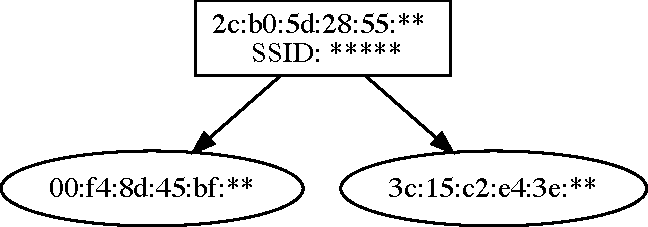
\includegraphics{images/img8censored.pdf}
	\caption{Primo esempio}
	\label{fig:es1}
\end{figure}


Nel grafo \ref{fig:es2} si mostra l'evoluzione topologica della stessa rete in un diverso momento della giornata, in questo caso si pu\`o notare la presenza di diversi nuovi dispositivi collegati.
%nonna3.pcap
\begin{figure}[!h]
	\centering
	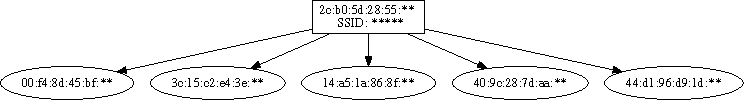
\includegraphics{images/img9censored.pdf}
	\caption{Secondo esempio}
	\label{fig:es2}
\end{figure}

La scelta di queste catture come primo esempio \'e riconducibile non solo alla semplice struttura della rete ma anche ad una semplicit\`a del traffico analizzato.
Una veloce analisi dei pacchetti catturati effettuata con il software Wireshark mostra, infatti, l'uso esclusivo di indirizzi MAC globalmente assegnati unicast e nessun tipo di repeater collegato alla rete.
Inoltre, l'access point utilizza un singolo indirizzo MAC: sia per effettuare le operazioni di annuncio di rete tramite frame beacon che per interagire con i dispositivi connessi.

Una prima validazione delle euristiche utilizate pu\`o essere invece vista nella figura \ref{fig:es3}.
Il numero di dispositivi \'e di nuovo limitato ma in questo caso, analizzando i pacchetti catturati, si pu\`o notare la presenza di diversi indirizzi MAC legati al router ed un uso di indirizzi multicast.
Il beacon frame della rete in esame viene infatti trasmesso attraverso l'uso di un indirizzo localmente assegnato, mentre le operazioni come trasmissione di frame data vengono effettuate utilizzando l'effettivo indirizzo MAC del dispositivo.
Una particolarit\`a di questa topologia \'e nell'utilizzo di indirizzi multicast dei dispositivi collegati per l'invio di frame di tipo controllo che vengono correttamente gestiti dalla libreria sviluppata.

%Fermo - Multicast

\begin{figure}[!h]
	\centering
	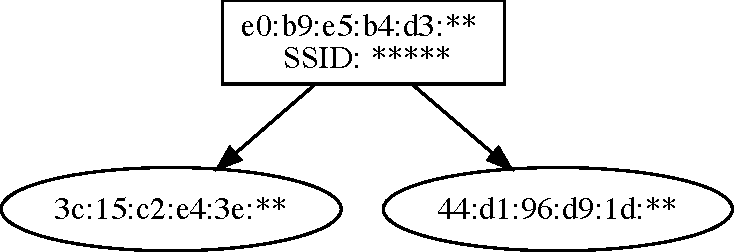
\includegraphics{images/img10censored.pdf}
	\caption{Terzo esempio}
	\label{fig:es3}
\end{figure}


L'ultima cattura presentata per questa sezione in figura \ref{fig:es4} proviene da una rete 5G i cui dispositivi connessi sono principalmente smartphone e smart speaker quali Google Home.
Data la possibilit\`a di questo router di operare simultaneamente in dual-band, annunciando quindi reti in 2G e 5G, le euristiche implementate sono fondamentali per gestire i numerosi indirizzi MAC localmente assegnati che operano nelle due diverse bande.
Questo tipo di cattura mostra anche come la soluzione proposta sia in grado di identificare dispositivi spesso inattivi, quali smart speaker, con un minimo traffico di rete. 


\begin{figure}[!h]
	\centering
	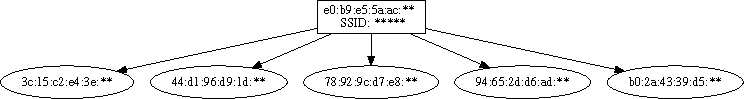
\includegraphics{images/img11censored.pdf}
	\caption{Quarto esempio}
	\label{fig:es4}
\end{figure}

%Casa

\newpage

\subsubsection{Reti con repeater}

Per la validazione su reti con topologia pi\`u complessa sono stati effettuate delle prove con diversi repeater Wi-Fi.

Il primo esempio che si riporta in figura \ref{fig:es5} riguarda l'introduzione di un repeater in una rete gi\`a presentata.
Il traffico analizzato mostra come, in questo caso, il repeater agisca in maniera "trasparente", aggiungendo il suo indirizzo MAC come trasmettitore nei frame riguardanti i dispositivi a lui connesso.
In aggiunta nella rete \'e presente un dispositivo di tipo IoT che, oltre ad interagire con i dispositivi interni, effettua annunci della propria rete locale.
%CasaRepeater

\begin{figure}[!h]
	\centering
	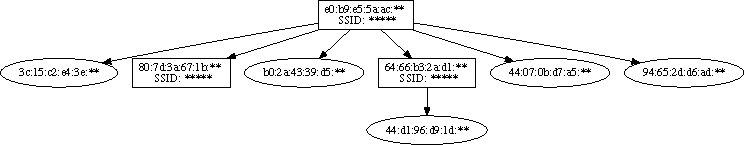
\includegraphics{images/img12censored.pdf}
	\caption{Quinto esempio}
	\label{fig:es5}
\end{figure}


Si presenta ora una delle catture pi\`u significative per la validazione della soluzione proposta.
La rete in esame in figura \ref{fig:es6} \'e composta da un router collegato tramite cavo ad un access point che fornisce connettivit\`a Wi-Fi.
A sua volta a questo viene collegato un repeater che verr\`a utilizzato dai dispositivi per usufruire della connessione.

\begin{figure}[!h]
	\centering
	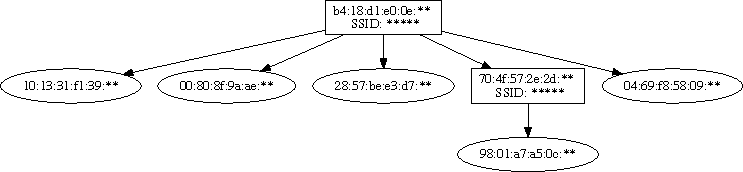
\includegraphics{images/img13censored.pdf}
	\caption{Sesto esempio}
	\label{fig:es6}
\end{figure}
%Wifi_repeater

Il repeater utilizzato in questa configurazione, pur differendo da quello presentato nel precedente esempio solo per il firmware in uso, ha un comportamento totalmente diverso.
Vengono utilizzati un numero di indirizzi MAC localmente assegnati pari al numero di dispositivi a lui collegati il cui valore \'e pari ad una composizione del LAA del repeater e del NIC del dispositivo.
Le euristiche presentate nel precedente capitolo riescono, come mostrato in figura, a classificare correttamente questo scenario.
I valori To DS e From DS presentati nel capitolo precedente permettono, inoltre, di identificare il collegamento tra router ed access point come cablato.
Infatti, dall'analisi del traffico, si pu\`o notare un cambio di mezzo trasmissivo tra access point e router ed un una mancanza di quest'ultimo di metriche Wi-Fi.

L'ultimo esempio che si riporta in figura \ref{fig:es7} riguarda un'altra rete locale con la presenza di repeater che non utilizza indirizzi localmente assegnati per la gestione dei dispositivi a lui connessi.
  
\begin{figure}[!h]
	\centering
	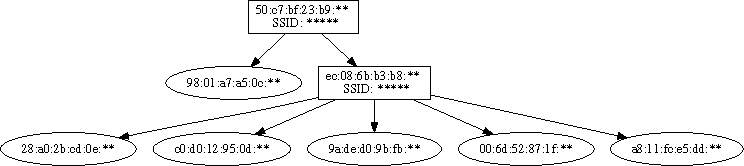
\includegraphics{images/img14censored.pdf}
	\caption{Settimo esempio}
	\label{fig:es7}
\end{figure}

\subsubsection{Reti complesse}
Sebbene la libreria per la ricostruzione della topologia Wi-Fi sia stata sviluppata per un funzionamento su reti locali domestiche sono state effettuate anche delle prove su reti professionali di medie dimensioni.
In questo caso, poich\`e non si conosce l'effettiva topologia della rete, non si \'e in grado di determinare l'efficacia della soluzione proposta se non constatando la presenza di dispositivi personali collegati.
Queste prove hanno per\`o mostrato come la libreria sia in grado di distinguere tra diversi SSID annunciati dallo stesso dispositivo di rete, una peculiarit\`a presente in access point di fascia alta.


\begin{figure}[!h]
	\centering
	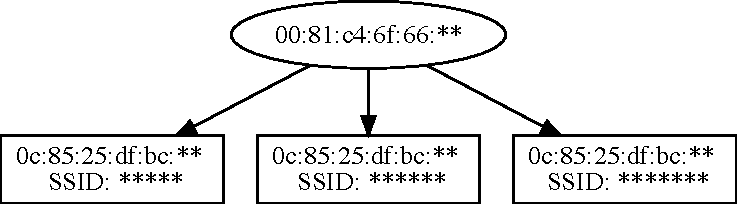
\includegraphics{images/img15censored.pdf}
	\caption{Ottavo esempio}
	\label{fig:es8}
\end{figure}

%Biblioteca
\newpage 

\section{Rilevazione di disservizi}

Le metriche di qualit\`a della connettivit\`a  che utilizza la soluzione proposta sono due:
\begin{itemize}
	\item RTT: ottenuto tramite l'ARP scan, se effettuata.
	\item SNR: ottenuto effettuando la differenza tra potenza segnale Wi-Fi e rumore di sottofondo.
\end{itemize}

Il RTT ottenuto nella rete \'e utile per fornire un quadro generale della raggiungibilit\`a di tutti i dispositivi collegati alla rete locale sotto analisi ma non \'e particolarmente utile alla rilevazione di disservizi per dispositivi Wi-Fi.
%Eth vs Wifi

Questa metrica \'e per\`o l'unica utilizzata dalla soluzione proposta per valutare lo stato di connessione di dispositivi cablati, rendendo quindi fondamentale l'uso dell'ARP scan se si desidera conoscere la connettivit\`a di questi terminali.

I valori considerati standard per questo tipo di analisi sono <1ms per quanto riguarda la connessione cablata mentre questa metrica si rileva poco efficace per stimare una connettivit\`a di tipo wireless, poich\`e troppo inconsistente.

Per fornire una pi\`u accurata misura della bont\`a del segnale la soluzione proposta, come introdotto nel capitolo precedente, dopo aver ottenuto i parametri di potenza del segnale e rumore di sottofondo, calcola il SNR.
Questo tipo di metrica, utilizzata dai network manager di tutti i sistemi operativi e software professionali, fornisce una divisione in categorie della bont\`a del segnale.

Poich\`e i valori utilizzati dal calcolo vengono calcolati in base alla potenza del segnale alla scheda di rete che sta effettuando la cattura dei frame, il dispositivo implementante la soluzione proposta deve essere posto in prossimit\`a dell'access point della rete che si vuole monitorare.

Utilizzando la topologia ottenuta dall'analisi dei frame ed i SNR calcolati la libreria \'e in grado di identificare in modo esatto, in caso di problemi di connessione Wi-Fi, tutti i dispositivi affetti.
Questo \'e possibile sia nel caso in cui il dispositivo \'e connesso direttamente all'access point e sia quando il dispositivo \'e connesso ad un repeater.

Nel primo caso, un valore non ottimale del SNR, identifica un problema nel dispositivo stesso poich\`e esso \'e direttamente collegato all'access point.
Nel secondo caso, poich\`e si conosce anche il valore SNR del repeater collegato all'access point, un valore non ottimale in questo dispositivo avr\`a ripercussioni anche sulla connessione dei terminali a lui collegato.
In questo caso i valori SNR di quest'ultimi si riferiscono al loro collegamento con il repeater.

In questi modi, se un dispositivo ha un SNR <15db, la sua connessione e quella di  terminali a lui eventualmente connessi vengono considerate affette da disservizi.

%\newpage

\section{Analisi delle prestazioni}

Poich\`e si vuole implementare la soluzione proposta su dispositivi con limitate risorse di memoria e calcolo, come ad esempio router, \'e importante fornire un'implementazione che non sia eccessivamente dispendiosa sotto questi due tipi di metriche.

Le strutture utilizzate per l'analisi ed i relativi dati memorizzati sono stati introdotti nel capitolo precedente e dipendono fortemente dal numero di dispositivi identificati con l'analisi del traffico.
Bench\`e questi siano generalmente in basso numero in reti locali domestiche, la loro memorizzazione non \'e il principale dispendio di memoria che la libreria effettua.

Mediante il software per la ricerca di problemi di memoria Valgrind \cite{valgrind}, ci si \'e assicurati che la libreria sviluppata non presenti memory leak e, utilizzando i file di cattura precedentemente introdotti, se ne \'e analizzato l'utilizzo di memoria.

Utilizzando come riferimento i file di cattura presentati l'utilizzo di memoria medio della libreria \'e di circa 5MB.
L'utilizzo massimo di memoria \'e stato di circa 20MB ed \'e dovuto ad un lungo periodo di cattura e la presenza di un dispositivo in riproduzione streaming multimediale.
In questo caso il numero di pacchetti analizzati era circa 30 mila, una cifra ben lontana da catture effettuate per tempi ragionevoli anche in reti professionali con numerosissimi dispositivi connessi dove il numero di pacchetti analizzato \'e stato circa 4 mila.

Se ne pu\`o quindi dedurre che l'utilizzo di memoria della libreria \'e principalmente determinato dal numero di dispositivi connessi e dalla quantit\`a di traffico da loro generato.
La durata di cattura pu\`o comunque essere modificata in base alla quantit\`a di frame che vengono ricevuti.

Il tempo di esecuzione della libreria \'e strettamente legato alla durata della cattura di frame 802.11.
Anche in questo caso, le operazioni di analisi dei pacchetti implementate non sono, in ordine di tempo, dispendiose.

\chapter{Lavori futuri}

Nei capitoli precedenti sono state presentate e validate alcune euristiche implementate per la ricostruzione topologica di una rete Wi-Fi.
L'approccio utilizzato si basa sulle caratteristiche degli indirizzi MAC per identificare e raggruppare tutte le varie antenne che un router o repeater utilizzano per la trasmissione nella rete locale.

Un possibile sviluppo futuro potrebbe essere quello di studiare ed eventualmente implementare diversi tipi di euristiche aggiuntive.
In particolare, una delle euristiche considerate durante il periodo di tirocinio riguarda l'uso che dispositivi quali router e repeater fanno di canali wireless.
Poich\`e questi sono forniti di numerose antenne, l'uso di un unico canale porterebbe ad una diminuzione della bont\`a del segnale.
Studiando quindi il funzionamento di diverse tipologie di questi dispositivi si potrebbe implementare un'euristica che aiuti nel raggruppare tutti i vari indirizzi MAC e relative antenne in base al canale utilizzato.

Dopo aver validato la soluzione proposta su reti locali di piccole dimensioni si potrebbe estendere l'utilizzo di questa anche a reti professionali di dimensioni superiori.
Questo \'e infatti possibile posizionando una moltitudine di dispositivi implementanti la soluzione proposta nei pressi dei vari access point presenti in una rete di queste dimensioni.
Le modifiche da effettuare necessarie per il corretto funzionamento comprendono la realizzazione di un unico database a cui i vari dispositivi che effettuano monitoraggio  inviano, in maniera concorrente, la loro visione parziale della topologia e valori di bont\`a del segnale.
In questo modo \'e possibile analizzare tutto il traffico catturato dai dispositivi e ricostruire in modo dettagliato la topologia di una rete di grandi dimensioni.
Questo tipo di sviluppo comporta quindi una modifica sia architetturale che implementativa della soluzione proposta.

Estendendo sulla possibile implementazione precedentemente discussa la libreria di ricostruzione topologica potrebbe inoltre essere migliorata implementando un' analisi di frame inviati da un distribution system ad un altro.
Questo tipo di frame sono utilizzati in reti di tipo wireless distribution system (WDS), un sistema che permette l'interazione tra due reti wireless diverse.

Si possono effettuare anche migliorie per fornire informazioni pi\`u specifiche sui dispositivi all'interno della rete.

Una di queste sarebbe l'implementazione di funzioni che, tramite un database di indirizzi, ricerchino i primi tre ottetti dell'indirizzo MAC, ovvero l' OUI, per stabilire il produttore del dispositivo rilevato.

In aggiunta, concentrandosi sulla rete locale che si vuole analizzare, \'e possibile scoprire servizi offerti dai dispositivi connessi attraverso DNS-based Service Discovery (DNS-SD) \cite{rfc6763}.
Nelle reti domestiche, dove magari non \'e presente un server DNS centrale, questo tipo di operazione pu\`o essere svolta mediante il protocollo mDNS\cite{rfc6762}.

Le informazioni ottenute possono poi essere utilizzate per modellare il minimo valore SNR in modo specifico al tipo di dispositivo.
Ad esempio, un dispositivo come una smart TV che annuncia in rete un servizio di streaming, necessita di una connessione molto affidabile rispetto ad altri dispositivi che, magari, non utilizzano costantemente la connessione di rete.

Infine, sempre restando in un ottica di analisi di una rete locale specifica, sarebbe utile fornire un'analisi del traffico TCP della rete in modo da poter analizzare, ad esempio, il numero di ritrasmissioni e pacchetti persi.

\chapter{Conclusione}


\backmatter
\emergencystretch=1em
\printbibliography[heading=bibintoc]

\begin{appendices}
\addtocontents{toc}{\protect\enlargethispage{2\baselineskip}}
\chapter{Codice sorgente}

Il codice sorgente sviluppato durante l'attivit\`a di tirocinio pu\`o essere trovato alla seguente pagina:

\url{https://github.com/dcasenove/WiFi-Topology}

\end{appendices}
\end{document}